\chapter{Acoustic Heterodyning}
\label{ch:acoustic-heterodyning}

\begin{nontechnical}
\textbf{Imagine mixing colors}---when you mix blue and yellow paint, you get green. Acoustic heterodyning is similar, but with sound waves.

\textbf{The basic idea:}
\begin{itemize}
\item Take two ultrasound beams (too high-pitched for humans to hear, like dog whistles)
\item Aim them at the same spot
\item When they overlap, they ``mix'' together in a nonlinear way
\item This creates a new, audible sound at the \emph{difference} between their frequencies
\end{itemize}

\textbf{Real-world example:} If you send 40,000~Hz and 42,000~Hz ultrasound beams (both inaudible), they can create a 2,000~Hz tone (clearly audible) where they meet.

\textbf{Why this matters:} Museums use directional speakers that beam sound to just one person. Doctors use it for clearer ultrasound images. Scientists are exploring brain stimulation applications.

\textbf{The catch:} Only about 0.1--1\% of the ultrasound energy converts to audible sound, so you need powerful sources.
\end{nontechnical}

\section{Overview}

\textbf{Acoustic heterodyning} (also called parametric acoustic arrays) exploits \textbf{nonlinear acoustics} to generate new frequencies through wave mixing. When two ultrasound beams at frequencies $f_1$ and $f_2$ interact in a nonlinear medium, they produce a difference frequency $f_\Delta = |f_1 - f_2|$ that can be in the audible range.

\begin{keyconcept}
The key principle: \textbf{Nonlinear wave propagation} causes high-frequency ultrasound beams to interact and generate lower-frequency components. This enables highly directional low-frequency sound without requiring large transducer arrays.
\end{keyconcept}

\textbf{Established applications:}
\begin{itemize}
\item Parametric loudspeakers for directional audio
\item Underwater sonar systems
\item Medical harmonic imaging
\end{itemize}

\textbf{Emerging research:}
\begin{itemize}
\item Neural stimulation via focused ultrasound heterodyning
\item Targeted drug delivery using acoustic pressure modulation
\end{itemize}

\section{Mathematical Description}

\subsection{Nonlinear Wave Equation}

The fundamental physics of acoustic heterodyning is described by the \textbf{Westervelt equation}, which includes nonlinear acoustic propagation:
\begin{equation}
\frac{\partial^2 p}{\partial t^2} - c^2 \nabla^2 p = \frac{\beta}{\rho_0 c^2} \frac{\partial^2 (p^2)}{\partial t^2}
\end{equation}
where:
\begin{itemize}
\item $p$ = acoustic pressure (Pa)
\item $c$ = speed of sound in medium (m/s)
\item $\beta$ = coefficient of nonlinearity (dimensionless)
\item $\rho_0$ = equilibrium density of medium (kg/m$^3$)
\end{itemize}

The right-hand side term represents the \textbf{nonlinear source} that enables frequency mixing.

\subsection{Two-Tone Interaction}

For two incident ultrasound waves:
\begin{equation}
p_{\text{in}}(t) = p_1 \cos(\omega_1 t) + p_2 \cos(\omega_2 t)
\end{equation}
where:
\begin{itemize}
\item $p_1, p_2$ = pressure amplitudes of primary waves (Pa)
\item $\omega_1, \omega_2$ = angular frequencies (rad/s)
\item $f_1 = \omega_1/(2\pi)$ and $f_2 = \omega_2/(2\pi)$ (Hz)
\end{itemize}

The nonlinear term $p^2$ expands to:
\begin{equation}
p^2 = p_1^2\cos^2(\omega_1 t) + p_2^2\cos^2(\omega_2 t) + 2p_1 p_2 \cos(\omega_1 t)\cos(\omega_2 t)
\end{equation}

Using the trigonometric product identity:
\begin{equation}
\cos A \cos B = \frac{1}{2}[\cos(A-B) + \cos(A+B)]
\end{equation}

The cross-term generates:
\begin{equation}
2p_1 p_2 \cos(\omega_1 t)\cos(\omega_2 t) = p_1 p_2[\cos(\omega_1 - \omega_2)t + \cos(\omega_1 + \omega_2)t]
\end{equation}
where:
\begin{itemize}
\item $\omega_\Delta = \omega_1 - \omega_2$ = difference frequency (rad/s)
\item $\omega_\Sigma = \omega_1 + \omega_2$ = sum frequency (rad/s)
\end{itemize}

\begin{keyconcept}
The \textbf{difference frequency} $f_\Delta = |f_1 - f_2|$ can be in the audible range (20~Hz--20~kHz) even when $f_1$ and $f_2$ are ultrasonic ($>$20~kHz). The sum frequency $f_\Sigma$ is even higher and typically heavily attenuated.
\end{keyconcept}

\subsection{Difference Frequency Amplitude}

The amplitude of the generated difference frequency is:
\begin{equation}
p_\Delta = \frac{\beta k_1 k_2 p_1 p_2 L}{4 \rho_0 c^2}
\end{equation}
where:
\begin{itemize}
\item $p_\Delta$ = pressure amplitude at difference frequency (Pa)
\item $k_1 = 2\pi f_1/c$, $k_2 = 2\pi f_2/c$ = wavenumbers (rad/m)
\item $L$ = interaction length (m)
\end{itemize}

\textbf{Key observation:} The difference frequency amplitude is proportional to:
\begin{itemize}
\item The product $p_1 p_2$ (both primaries must be present)
\item The interaction length $L$ (longer overlap = stronger mixing)
\item The nonlinearity parameter $\beta$ (material property)
\end{itemize}

\subsection{Efficiency}

The power conversion efficiency is defined as:
\begin{equation}
\eta = \frac{P_\Delta}{P_1 + P_2}
\end{equation}
where:
\begin{itemize}
\item $\eta$ = conversion efficiency (dimensionless)
\item $P_\Delta$ = acoustic power at difference frequency (W)
\item $P_1, P_2$ = acoustic power of primary beams (W)
\end{itemize}

Typical values: $\eta \approx 0.001$ to $0.01$ (0.1\% to 1\%)

\begin{calloutbox}{Why So Inefficient?}
Acoustic heterodyning is inherently inefficient because:
\begin{enumerate}
\item The nonlinear term $\beta$ is small (typically 3--10)
\item Pressure amplitudes must remain below cavitation thresholds
\item Absorption losses increase with frequency
\item The interaction length is limited by beam divergence
\end{enumerate}
Despite low efficiency, the technique is valuable for its unique directional properties.
\end{calloutbox}

\subsection{Nonlinearity Parameter Values}

Different media exhibit different degrees of nonlinearity:
\begin{equation}
\beta_{\text{tissue}} > \beta_{\text{water}} > \beta_{\text{air}}
\end{equation}

\textbf{Representative values:}

\begin{center}
\begin{tabular}{@{}lc@{}}
\toprule
\textbf{Medium} & $\beta$ \\
\midrule
Air & 1.2 \\
Water (20°C) & 5.0 \\
Seawater & 5.25 \\
Muscle tissue & 5.5 \\
Liver tissue & 6.5 \\
Fat tissue & 10.0 \\
\bottomrule
\end{tabular}
\end{center}

\section{Heterodyning Process Diagram}

The acoustic heterodyning process can be visualized as follows:

\begin{center}
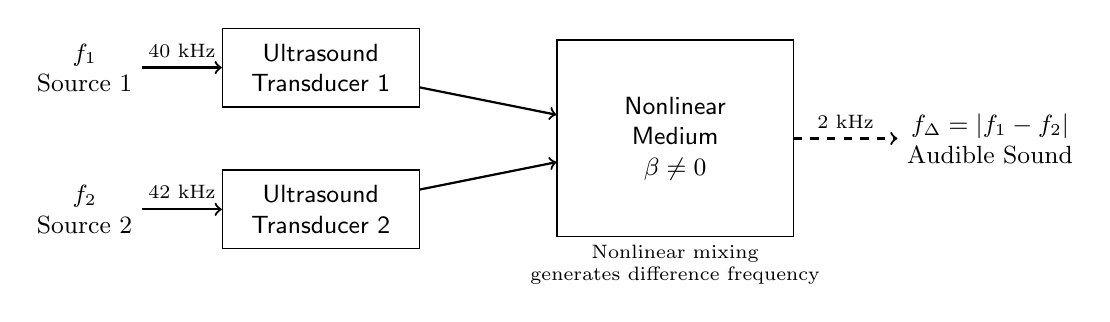
\begin{tikzpicture}[
  block/.style={rectangle, draw, minimum width=2.5cm, minimum height=1cm, font=\sffamily\small, align=center},
  node distance=2.5cm,
  font=\small
]
\node[align=center] (source1) {\sffamily $f_1$\\Source 1};
\node[block, right of=source1, node distance=3cm] (trans1) {Ultrasound\\Transducer 1};
\node[below of=source1, node distance=1.8cm, align=center] (source2) {\sffamily $f_2$\\Source 2};
\node[block, right of=source2, node distance=3cm] (trans2) {Ultrasound\\Transducer 2};

\node[block, right of=trans1, node distance=4.5cm, yshift=-0.9cm, minimum width=3cm, minimum height=2.5cm] (medium) {Nonlinear\\Medium\\$\beta \neq 0$};

\node[right of=medium, node distance=4cm, align=center] (output) {\sffamily $f_\Delta = |f_1 - f_2|$\\Audible Sound};

% Arrows
\draw[->,thick] (source1) -- node[above,font=\scriptsize] {40~kHz} (trans1);
\draw[->,thick] (source2) -- node[above,font=\scriptsize] {42~kHz} (trans2);
\draw[->,thick] (trans1) -- (medium);
\draw[->,thick] (trans2) -- (medium);
\draw[->,thick,dashed] (medium) -- node[above,font=\scriptsize] {2~kHz} (output);

% Labels
\node[below of=medium, node distance=1.6cm, font=\scriptsize, align=center] {Nonlinear mixing\\generates difference frequency};
\end{tikzpicture}
\end{center}

\subsection{Frequency Spectrum}

The nonlinear interaction generates multiple frequency components:

\begin{center}
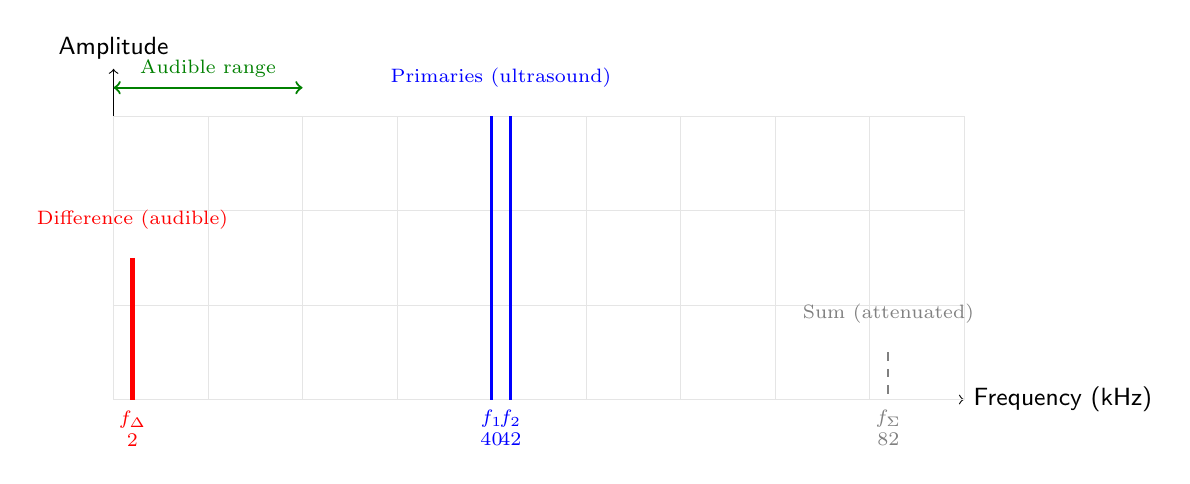
\begin{tikzpicture}[scale=1.2]
% Axes
\draw[->] (0,0) -- (9,0) node[right,font=\sffamily\small] {Frequency (kHz)};
\draw[->] (0,0) -- (0,3.5) node[above,font=\sffamily\small] {Amplitude};

% Grid
\draw[very thin,gray!20] (0,0) grid[step=1] (9,3);

% Primary frequencies (40 kHz, 42 kHz scaled down for display)
\draw[thick,blue] (4,3) -- (4,0) node[below,font=\scriptsize,blue,align=center] {$f_1$\\40};
\draw[thick,blue] (4.2,3) -- (4.2,0) node[below,font=\scriptsize,blue,align=center] {$f_2$\\42};

% Difference frequency (2 kHz)
\draw[thick,red,line width=1.5pt] (0.2,1.5) -- (0.2,0) node[below,font=\scriptsize,red,align=center] {$f_\Delta$\\2};

% Sum frequency (82 kHz - off scale)
\draw[thick,gray,dashed] (8.2,0.5) -- (8.2,0) node[below,font=\scriptsize,gray,align=center] {$f_\Sigma$\\82};

% Labels
\node[above,font=\scriptsize,blue] at (4.1,3.2) {Primaries (ultrasound)};
\node[above,font=\scriptsize,red] at (0.2,1.7) {Difference (audible)};
\node[above,font=\scriptsize,gray] at (8.2,0.7) {Sum (attenuated)};

% Audible range indicator
\draw[<->,thick,green!50!black] (0,3.3) -- (2,3.3) node[midway,above,font=\scriptsize] {Audible range};
\end{tikzpicture}
\end{center}

The difference frequency $f_\Delta = 2$~kHz falls within the audible range, while the sum frequency $f_\Sigma = 82$~kHz is rapidly absorbed.

\section{Applications}

\subsection{Parametric Loudspeakers}

\textbf{Principle:} Ultrasound beams (e.g., 40~kHz carrier) are highly direc\-tion\-al ($\sim$5\textdegree{} beamwidth). The audible difference frequency inherits this directionality, creating a ``beam of sound.''

\begin{center}
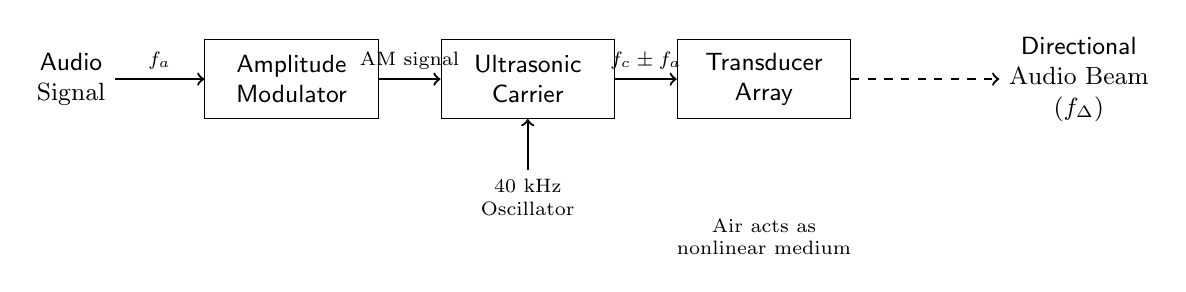
\begin{tikzpicture}[
  block/.style={rectangle, draw, minimum width=2.2cm, minimum height=1cm, font=\sffamily\small, align=center},
  node distance=2.2cm,
  font=\small
]
\node[align=center] (input) {\sffamily Audio\\Signal};
\node[block, right of=input, node distance=2.8cm] (mod) {Amplitude\\Modulator};
\node[block, right of=mod, node distance=3cm] (carrier) {Ultrasonic\\Carrier};
\node[block, right of=carrier, node distance=3cm] (array) {Transducer\\Array};
\node[right of=array, node distance=4cm, align=center] (output) {\sffamily Directional\\Audio Beam\\($f_\Delta$)};

% Arrows
\draw[->,thick] (input) -- node[above,font=\scriptsize] {$f_a$} (mod);
\draw[->,thick] (mod) -- node[above,font=\scriptsize] {AM signal} (carrier);
\draw[->,thick] (carrier) -- node[above,font=\scriptsize] {$f_c \pm f_a$} (array);
\draw[->,thick,dashed] (array) -- (output);

% Carrier source
\node[below of=carrier, node distance=1.5cm, font=\scriptsize, align=center] (osc) {40~kHz\\Oscillator};
\draw[->,thick] (osc) -- (carrier);

% Note
\node[below of=array, node distance=2cm, font=\scriptsize, align=center] {Air acts as\\nonlinear medium};
\end{tikzpicture}
\end{center}

\textbf{Commercial products:}
\begin{itemize}
\item \textbf{Audio Spotlight (Holosonics):} Museum exhibits, retail displays
\item \textbf{HyperSound (Turtle Beach):} Personal audio systems
\item \textbf{Sennheiser Audiobeam:} Conference room systems
\end{itemize}

\textbf{Advantages:}
\begin{itemize}
\item Highly directional low-frequency sound without large transducers
\item Minimal side lobes (sound stays in the beam)
\item Adjustable beam width via array geometry
\end{itemize}

\textbf{Limitations:}
\begin{itemize}
\item Low efficiency ($\sim$1\% conversion)
\item Nonlinear distortion (harmonics of audio signal)
\item Limited sound pressure level
\item High power consumption
\end{itemize}

\subsection{Medical Harmonic Imaging}

\textbf{Technique:} Transmit fundamental frequency $f_0$, receive second harmonic $2f_0$ generated by tissue nonlinearity.

The received harmonic signal is:
\begin{equation}
p_{2f_0} = \frac{\beta k^2 p_0^2 z}{8\rho_0 c^2}
\end{equation}
where:
\begin{itemize}
\item $p_{2f_0}$ = second harmonic pressure amplitude (Pa)
\item $k = 2\pi f_0/c$ = wavenumber at fundamental (rad/m)
\item $z$ = propagation distance (m)
\item $p_0$ = transmitted pressure amplitude (Pa)
\end{itemize}

\textbf{Clinical applications:}
\begin{itemize}
\item \textbf{Echocardiography:} Enhanced contrast, reduced artifacts
\item \textbf{Liver imaging:} Better lesion detection
\item \textbf{Contrast-enhanced ultrasound:} Microbubble agents enhance har\-mon\-ic response
\end{itemize}

\textbf{Advantages:}
\begin{itemize}
\item Improved resolution (shorter wavelength at $2f_0$)
\item Reduced clutter (harmonics generated only in nonlinear tissue)
\item Better signal-to-noise ratio in deep tissue
\end{itemize}

\subsection{Underwater Parametric Sonar}

\textbf{Parametric sonar} transmits high-frequency beams that generate direc\-tion\-al low-frequency sound through ocean nonlinearity.

The parametric array gain is:
\begin{equation}
G_{\text{PA}} = 20\log_{10}\left(\frac{f_1 + f_2}{2f_\Delta}\right)
\end{equation}
where:
\begin{itemize}
\item $G_{\text{PA}}$ = processing gain (dB)
\item $f_1, f_2$ = primary frequencies (Hz)
\item $f_\Delta$ = difference frequency (Hz)
\end{itemize}

\textbf{Applications:}
\begin{itemize}
\item Submarine communication (low-frequency propagates farther)
\item Bathymetric mapping (sub-bottom profiling)
\item Marine mammal deterrence (targeted acoustic signals)
\end{itemize}

\subsection{Neuromodulation Research}

\textbf{Hypothesis:} Two focused ultrasound beams at slightly different frequencies cross in brain tissue, generating a low-frequency pressure modulation that stimulates mechanosensitive ion channels.

The focal overlap region size is:
\begin{equation}
V_{\text{focus}} = \frac{4\pi}{3}\left(\frac{\lambda D}{4a}\right)^3
\end{equation}
where:
\begin{itemize}
\item $V_{\text{focus}}$ = focal volume (m$^3$)
\item $\lambda$ = wavelength (m)
\item $D$ = focal depth (m)
\item $a$ = aperture radius (m)
\end{itemize}

\textbf{Theoretical advantages:}
\begin{itemize}
\item Spatial selectivity (only overlap region affected)
\item Tunable frequency (can match neural response frequencies)
\item Non-invasive delivery
\end{itemize}

\textbf{Challenges:}
\begin{itemize}
\item \textbf{Low efficiency:} Requires high intensity ($>$1~W/cm$^2$) $\rightarrow$ safety concerns
\item \textbf{Skull distortion:} Requires adaptive focusing or cranial windows
\item \textbf{Mechanism unclear:} Thermal vs. mechanical effects debated
\end{itemize}

\textbf{Experimental status:}
\begin{itemize}
\item \emph{In vitro:} Calcium signaling observed (Ye et al., 2018)
\item \emph{In vivo:} Behavioral changes in rodents (mechanism debated)
\item \emph{Humans:} No transcranial studies published
\end{itemize}

\begin{warningbox}
Transcranial acoustic heterodyning for human neuromodulation remains \textbf{experimental and unproven}. Safety limits for chronic ultrasound exposure to brain tissue are not well established. Any clinical application requires rigorous FDA approval.
\end{warningbox}

\section{Performance Analysis}

\subsection{Beam Pattern and Directivity}

The beam pattern of a parametric array is governed by:
\begin{equation}
D(\theta) = \frac{\sin(ka\sin\theta)}{ka\sin\theta}
\end{equation}
where:
\begin{itemize}
\item $D(\theta)$ = directivity function (dimensionless)
\item $k = 2\pi f/c$ = wavenumber (rad/m)
\item $a$ = transducer radius (m)
\item $\theta$ = angle from acoustic axis (rad)
\end{itemize}

The $-3$~dB beamwidth is approximately:
\begin{equation}
\theta_{-3\text{dB}} \approx 1.02 \frac{\lambda}{D_{\text{aperture}}} = 1.02 \frac{c}{f D_{\text{aperture}}}
\end{equation}
where:
\begin{itemize}
\item $\theta_{-3\text{dB}}$ = half-power beamwidth (radians)
\item $D_{\text{aperture}}$ = aperture diameter (m)
\end{itemize}

\textbf{Example:} For 40~kHz ultrasound with 10~cm aperture in air ($c = 343$~m/s):
\begin{equation}
\theta_{-3\text{dB}} = 1.02 \times \frac{343}{40{,}000 \times 0.1} \approx 0.087~\text{rad} = 5°
\end{equation}

\subsection{Absorption and Propagation Distance}

The absorption coefficient for ultrasound in air is:
\begin{equation}
\alpha_{\text{air}} \approx 1.6 \times 10^{-10} f^2 \quad \text{(Np/m at 20°C)}
\end{equation}
where:
\begin{itemize}
\item $\alpha_{\text{air}}$ = absorption coefficient (Nepers/m)
\item $f$ = frequency (Hz)
\end{itemize}

The effective range of a parametric array is:
\begin{equation}
R_{\text{eff}} \approx \frac{1}{2\alpha_1 + 2\alpha_2}
\end{equation}
where:
\begin{itemize}
\item $R_{\text{eff}}$ = effective range (m)
\item $\alpha_1, \alpha_2$ = absorption at primary frequencies (Np/m)
\end{itemize}

For 40~kHz in air: $R_{\text{eff}} \approx 10$--20~m (museum/retail applications)

\subsection{Safety Limits}

\textbf{FDA diagnostic ultrasound limits:}
\begin{equation}
I_{\text{SPTA}} < 720~\text{mW/cm}^2
\end{equation}
where:
\begin{itemize}
\item $I_{\text{SPTA}}$ = spatial-peak temporal-average intensity (mW/cm$^2$)
\end{itemize}

\textbf{Mechanical Index} (cavitation risk):
\begin{equation}
\text{MI} = \frac{p_{\text{neg}}}{\sqrt{f_{\text{MHz}}}} < 1.9
\end{equation}
where:
\begin{itemize}
\item MI = mechanical index (dimensionless)
\item $p_{\text{neg}}$ = peak negative pressure (MPa)
\item $f_{\text{MHz}}$ = frequency (MHz)
\end{itemize}

\textbf{Thermal Index} (heating risk):
\begin{equation}
\text{TI} = \frac{P_{\text{acoustic}}}{P_{\text{degrade}}} < 6
\end{equation}
where:
\begin{itemize}
\item TI = thermal index (dimensionless)
\item $P_{\text{acoustic}}$ = acoustic power (W)
\item $P_{\text{degrade}}$ = power required for 1°C temperature rise (W)
\end{itemize}

\section{Worked Example: Parametric Speaker Design}

\textbf{Scenario:} Design a parametric loudspeaker for museum exhibit with 2~kHz audio at 10~m distance

\subsection*{Given Parameters}

\begin{tabular}{@{}ll@{}}
Target audio frequency & $f_a = 2{,}000$~Hz \\
Carrier frequency & $f_c = 40{,}000$~Hz \\
Distance & $R = 10$~m \\
Aperture diameter & $D = 10$~cm \\
Air temperature & $T = 20$°C \\
Ambient pressure & $P_0 = 101{,}325$~Pa \\
Speed of sound & $c = 343$~m/s \\
Nonlinearity parameter (air) & $\beta = 1.2$ \\
Air density & $\rho_0 = 1.2$~kg/m$^3$ \\
\end{tabular}

\subsection*{Step 1: Choose Primary Frequencies}

For single-sideband modulation:
\begin{equation}
f_1 = f_c = 40{,}000~\text{Hz}
\end{equation}
\begin{equation}
f_2 = f_c + f_a = 40{,}000 + 2{,}000 = 42{,}000~\text{Hz}
\end{equation}

Difference frequency: $f_\Delta = f_2 - f_1 = 2{,}000$~Hz \checkmark

\subsection*{Step 2: Calculate Beamwidth}

\begin{equation}
\theta_{-3\text{dB}} = 1.02 \times \frac{343}{40{,}000 \times 0.1} = 0.0875~\text{rad} = 5.0°
\end{equation}

At 10~m distance, beam diameter:
\begin{equation}
D_{\text{beam}} = 2R\tan(\theta/2) \approx 2 \times 10 \times 0.0438 = 0.88~\text{m}
\end{equation}

\subsection*{Step 3: Calculate Required Primary Pressures}

Target audio SPL: 70~dB = 0.063~Pa

Using the heterodyning equation with $L = 0.5$~m interaction length:
\begin{equation}
p_\Delta = \frac{\beta k_1 k_2 p_1 p_2 L}{4\rho_0 c^2}
\end{equation}

Wavenumbers:
\begin{equation}
k_1 = \frac{2\pi \times 40{,}000}{343} = 733~\text{rad/m}
\end{equation}
\begin{equation}
k_2 = \frac{2\pi \times 42{,}000}{343} = 769~\text{rad/m}
\end{equation}

Assuming $p_1 = p_2 = p_0$ (equal primaries):
\begin{equation}
0.063 = \frac{1.2 \times 733 \times 769 \times p_0^2 \times 0.5}{4 \times 1.2 \times 343^2}
\end{equation}

Solving for $p_0$:
\begin{equation}
p_0 = \sqrt{\frac{0.063 \times 4 \times 1.2 \times 343^2}{1.2 \times 733 \times 769 \times 0.5}} \approx 4.8~\text{Pa}
\end{equation}

\subsection*{Step 4: Calculate Required Acoustic Power}

Intensity for plane wave:
\begin{equation}
I = \frac{p_0^2}{2\rho_0 c} = \frac{4.8^2}{2 \times 1.2 \times 343} = 0.028~\text{W/m}^2
\end{equation}

Total power for 10~cm diameter aperture:
\begin{equation}
P = I \times A = 0.028 \times \pi(0.05)^2 = 2.2 \times 10^{-4}~\text{W} = 0.22~\text{mW}
\end{equation}

\subsection*{Step 5: Account for Absorption}

Absorption coefficient at 40~kHz:
\begin{equation}
\alpha = 1.6 \times 10^{-10} \times (40{,}000)^2 = 0.256~\text{Np/m}
\end{equation}

Attenuation over 10~m:
\begin{equation}
\text{Loss} = e^{-2\alpha R} = e^{-2 \times 0.256 \times 10} = e^{-5.12} = 0.006 = -22.3~\text{dB}
\end{equation}

Required source power (accounting for losses):
\begin{equation}
P_{\text{source}} = \frac{0.22~\text{mW}}{0.006} \approx 37~\text{mW}
\end{equation}

\begin{calloutbox}[colback=black!5!white,colframe=black]{Design Summary}
\textbf{Result: Feasible parametric speaker design}

\begin{tabular}{@{}ll@{}}
Primary frequencies & 40~kHz, 42~kHz \\
Audio frequency & 2~kHz \\
Beamwidth & 5° (highly directional) \\
Beam diameter at 10~m & 0.88~m \\
Required acoustic power & 37~mW \\
\end{tabular}

\textbf{Conclusion:} Low power requirements make this practical for battery-powered portable units. The narrow beam provides excellent spatial selectivity for targeted audio delivery.
\end{calloutbox}

\section{Advantages and Disadvantages}

\begin{center}
\begin{tabular}{@{}p{7cm}p{7cm}@{}}
\toprule
\textbf{Advantages} & \textbf{Disadvantages} \\
\midrule
Highly directional low-frequency sound & Very low efficiency (0.1--1\%) \\
No large transducer arrays required & High power consumption \\
Adjustable beam pattern & Nonlinear distortion \\
Minimal side lobes & Limited sound pressure level \\
Scalable to various applications & Frequency-dependent performance \\
Non-contact delivery & Absorption limits range \\
\bottomrule
\end{tabular}
\end{center}

\section{Summary}

\textbf{Acoustic heterodyning} exploits nonlinear wave propagation to generate audible difference frequencies from ultrasonic primaries. The technique enables highly directional audio without large arrays, but suffers from low efficiency.

\begin{center}
\begin{tabular}{@{}ll@{}}
\toprule
\textbf{Parameter} & \textbf{Value} \\
\midrule
Principle & Nonlinear acoustic mixing \\
Efficiency & 0.1--1\% \\
Typical frequencies & 40--42~kHz $\rightarrow$ 2~kHz \\
Beamwidth & 3--10° \\
Effective range (air) & 10--20~m \\
Nonlinearity ($\beta$, air) & 1.2 \\
Nonlinearity ($\beta$, tissue) & 5--10 \\
Applications & Audio, sonar, medical imaging \\
\bottomrule
\end{tabular}
\end{center}

\section{Further Reading}

\begin{itemize}
\item \textbf{Intermodulation Distortion in Biology}---general nonlinear mixing phenomena
\item \textbf{Frey Microwave Auditory Effect}---electromagnetic-to-acoustic conversion (different mechanism)
\item \textbf{Ultrasound Physics}---fundamental acoustic propagation
\item \textbf{Nonlinear Acoustics}---advanced mathematical treatment
\item \textbf{Medical Ultrasound Imaging}---clinical applications
\item \textbf{Sonar Systems}---underwater acoustic applications
\end{itemize}

\subsection*{Key References}

\begin{enumerate}
\item \textbf{Westervelt, P. J.} ``Parametric Acoustic Array.'' \emph{J. Acoust. Soc. Am.} 35, 535--537 (1963)---foundational theory
\item \textbf{Yoneyama, M. et al.} ``The Audio Spotlight: An Application of Nonlinear Interaction of Sound Waves.'' \emph{J. Acoust. Soc. Am.} 73, 1532--1536 (1983)---parametric speaker demonstration
\item \textbf{Duck, F. A.} ``Nonlinear Acoustics in Diagnostic Ultrasound.'' \emph{Ultrasound Med. Biol.} 28, 1--18 (2002)---tissue nonlinearity review
\item \textbf{Ye, P. P. et al.} ``Frequency Dependence of Ultrasound Neurostimulation.'' \emph{Neuron} 98, 1020--1030 (2018)---dual-frequency FUS neuromodulation
\end{enumerate}
